%%%%%%%%%%%%%%%%%%%%%%%%%%%%%%%%%%%%%%%%%
% Beamer Presentation
% LaTeX Template
% Version 1.0 (10/11/12)
%
% This template has been downloaded from:
% http://www.LaTeXTemplates.com
%
% License:
% CC BY-NC-SA 3.0 (http://creativecommons.org/licenses/by-nc-sa/3.0/)
%
%%%%%%%%%%%%%%%%%%%%%%%%%%%%%%%%%%%%%%%%%

%----------------------------------------------------------------------------------------
%	PACKAGES AND THEMES
%----------------------------------------------------------------------------------------
\documentclass{beamer}
\usepackage{amsmath, amsthm, amsfonts}
\usepackage{graphicx}
\usepackage{caption}
\usepackage{subcaption}

\mode<presentation> {

% The Beamer class comes with a number of default slide themes
% which change the colors and layouts of slides. Below this is a list
% of all the themes, uncomment each in turn to see what they look like.

%\usetheme{default}
%\usetheme{AnnArbor}
%\usetheme{Antibes}
%\usetheme{Bergen}
%\usetheme{Berkeley}
%\usetheme{Berlin}
%\usetheme{Boadilla}
%\usetheme{CambridgeUS}
%\usetheme{Copenhagen}
%\usetheme{Darmstadt}
%\usetheme{Dresden}
%\usetheme{Frankfurt}
%\usetheme{Goettingen}
%\usetheme{Hannover}
%\usetheme{Ilmenau}
%\usetheme{JuanLesPins}
%\usetheme{Luebeck}
\usetheme{Madrid}
%\usetheme{Malmoe}
%\usetheme{Marburg}
%\usetheme{Montpellier}
%\usetheme{PaloAlto}
%\usetheme{Pittsburgh}
%\usetheme{Rochester}
%\usetheme{Singapore}
%\usetheme{Szeged}
%\usetheme{Warsaw}

% As well as themes, the Beamer class has a number of color themes
% for any slide theme. Uncomment each of these in turn to see how it
% changes the colors of your current slide theme.

%\usecolortheme{albatross}
%\usecolortheme{beaver}
%\usecolortheme{beetle}
%\usecolortheme{crane}
%\usecolortheme{dolphin}
%\usecolortheme{dove}
%\usecolortheme{fly}
%\usecolortheme{lily}
%\usecolortheme{orchid}
%\usecolortheme{rose}
%\usecolortheme{seagull}
%\usecolortheme{seahorse}
%\usecolortheme{whale}
%\usecolortheme{wolverine}

%\setbeamertemplate{footline} % To remove the footer line in all slides uncomment this line
%\setbeamertemplate{footline}[page number] % To replace the footer line in all slides with a simple slide count uncomment this line

%\setbeamertemplate{navigation symbols}{} % To remove the navigation symbols from the bottom of all slides uncomment this line
}

\usepackage{graphicx} % Allows including images
\usepackage{booktabs} % Allows the use of \toprule, \midrule and \bottomrule in tables

%----------------------------------------------------------------------------------------
%	TITLE PAGE
%----------------------------------------------------------------------------------------

\title[Isotopic Approximation]{Isotopic Approximation} % The short title appears at the bottom of every slide, the full title is only on the title page

\author{wegatron} % Your name
\institute[ZJU] % Your institution as it will appear on the bottom of every slide, may be shorthand to save space
{
ZJU\\ % Your institution for the title page
\medskip
%%\textit{john@smith.com} % Your email address
}
\date{\today} % Date, can be changed to a custom date

\begin{document}

\begin{frame}
\titlepage % Print the title page as the first slide
\end{frame}

\begin{frame}
\frametitle{Overview} % Table of contents slide, comment this block out to remove it
\tableofcontents %Throughout your presentation, if you choose to use \section{} and \subsection{} commands, these will automatically be printed on this slide as an overview of your presentation
\begin{block}{Target}
Generate a triangle surface mesh within a tolerance volume $\Omega$, isotropic to the boundary components of $\Omega$ and with a low triangle count.
\end{block}
\begin{example}[Result]
  \begin{figure}[h]
    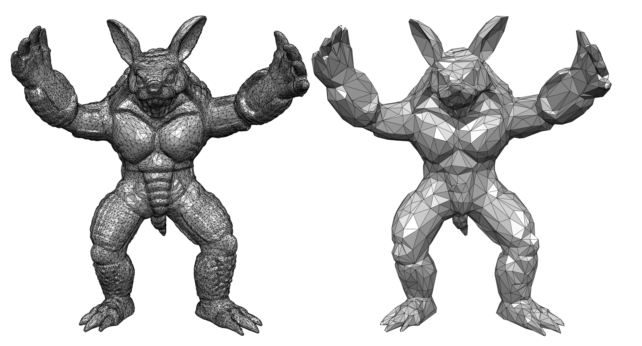
\includegraphics[width=6cm]{res}
  \end{figure}
\end{example}
\end{frame}

%----------------------------------------------------------------------------------------
%	PRESENTATION SLIDES
%----------------------------------------------------------------------------------------

%------------------------------------------------
%\section{First Section} % Sections can be created in order to organize your presentation into discrete blocks, all sections and subsections are automatically printed in the table of contents as an overview of the talk
%------------------------------------------------

%\subsection{Subsection Example} % A subsection can be created just before a set of slides with a common theme to further break down your presentation into chunks

\begin{frame}
\frametitle{Steps}
\begin{figure}[h]
  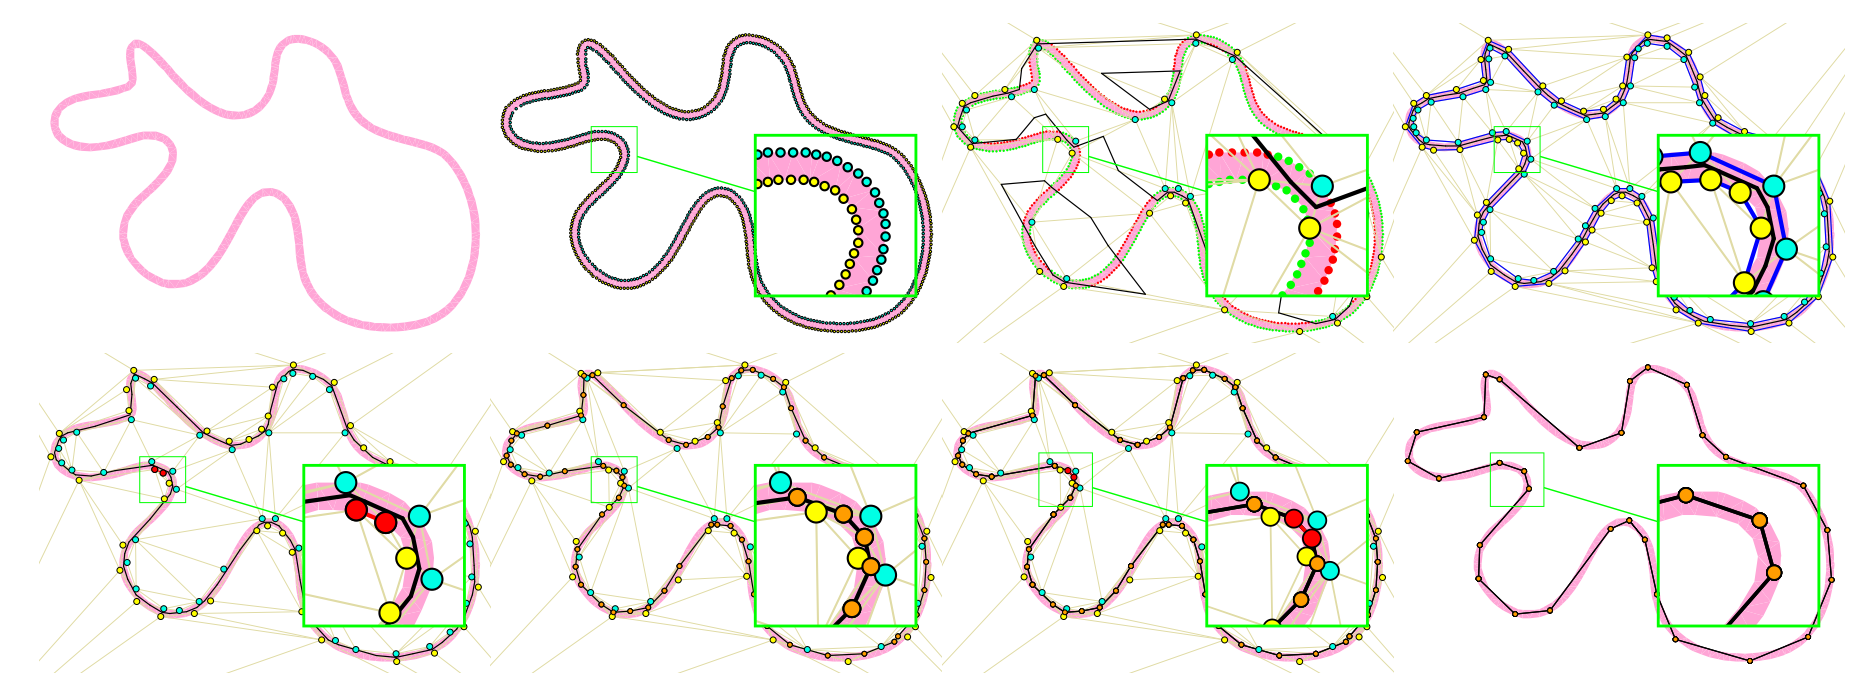
\includegraphics[width=8cm]{overview}
\end{figure}
\begin{itemize}
  \item Sampling: Generates a dense point sample S on the boundary of the tolerance volume $\partial \Omega$.
  \item Refine: select points from $\partial \Omega$ to construct $\Gamma$ -- a approximation of volume $\Omega$, By adding points to the triangulation $\tau$, until the piecewise-linear function $f(\mathtt{s})$ interpolated on $\tau$ is reliable enough.
  \item Simplification: Simplify the approximation volume $\partial \Gamma$, and the zero point set $\mathcal{Z}$(the final output), By do edge collapse.
\end{itemize}
\end{frame}

%------------------------------------------------

\begin{frame}
\frametitle{$\sigma$ Dense Sampling}
\begin{block}{Description}
Take sample points on a triangle, let all the circle(sample\_point, $\sigma$), can cover all the area of triangle.
\end{block}
\begin{block}{Procedure}
\begin{itemize}
  \item Transform the triangle into a local coordinate.
  \item Using $\sqrt{2} \sigma$ squares to cover the triangle left to right and botton to top, take the square's center as sample point.
  \item Transform back.
\end{itemize}
\end{block}
\begin{figure}[h]
  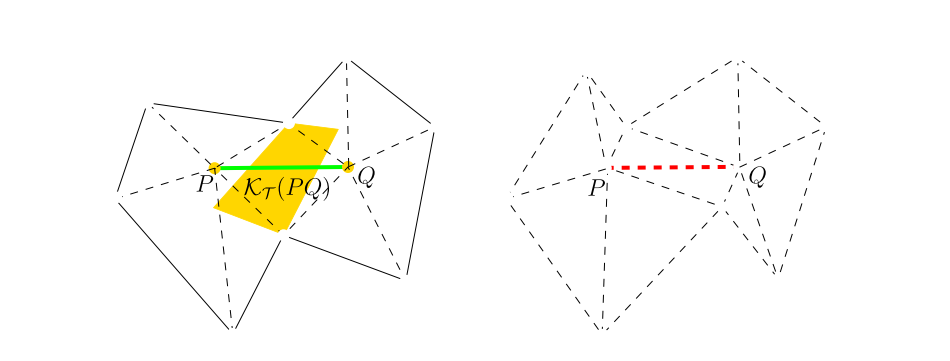
\includegraphics[width=6cm]{sampling}
\end{figure}
\end{frame}

%------------------------------------------------

\begin{frame}
\frametitle{Refine}
\begin{block}{Nature Idea}
  Greedily inserting the sample s with maximum error at each step, none of samples's error is bigger than 1.
\end{block}
\begin{block}{Two Modification}
   \begin{itemize}
     \item Error is should no more than $1-\alpha$. And we let $||f(s+\Delta s)-f(s)||<\alpha, \Delta s < \sigma$
     \item The tetrahedron t should classifies well the samples nearest to the vertices of shrunk copy of t.
   \end{itemize}
\end{block}
\begin{figure}[h]
  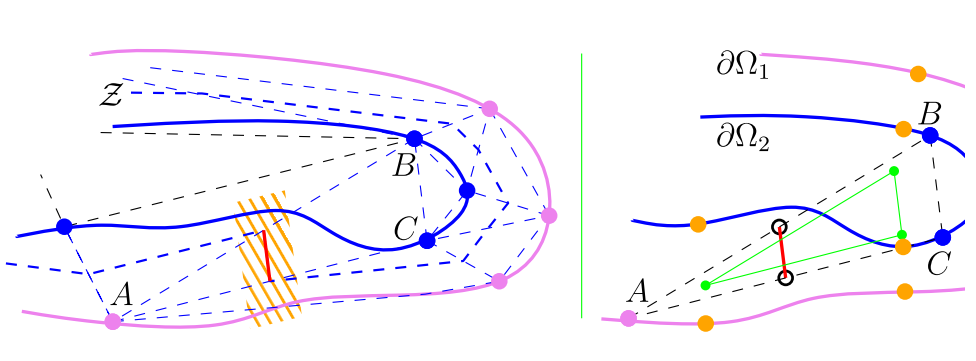
\includegraphics[width=6cm]{shrunk}
\end{figure}
\end{frame}

\begin{frame}
\frametitle{Simplification}
\begin{block}{Edge collapse on $\partial \Gamma$}
  \begin{itemize}
    \item Only merge two point into one.
    \item Target point in kernel area.
    \item The sample point in the area's error should no more than $1-\alpha$.
  \end{itemize}
\end{block}

\begin{figure}
  \centering
  \begin{subfigure}[b]{0.48\textwidth}
    \centering
    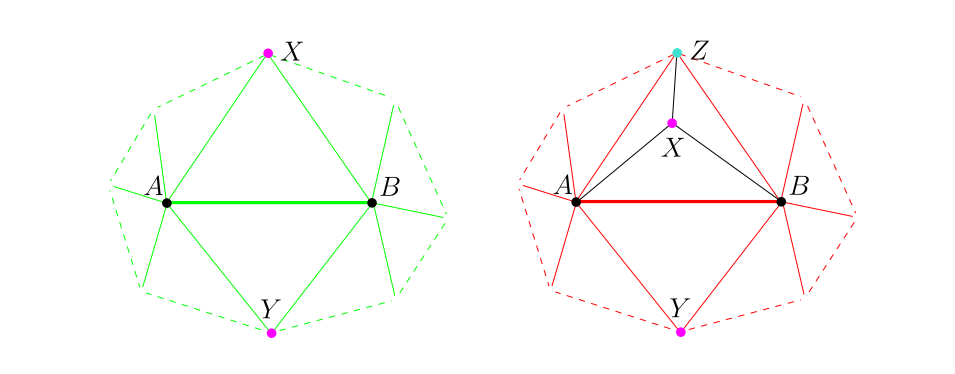
\includegraphics[width=\textwidth]{merge_two}
    \caption{merge two point into one}
    %\label{fig:y equals x}
  \end{subfigure}
  \hfill
  \begin{subfigure}[b]{0.48\textwidth}
    \centering
    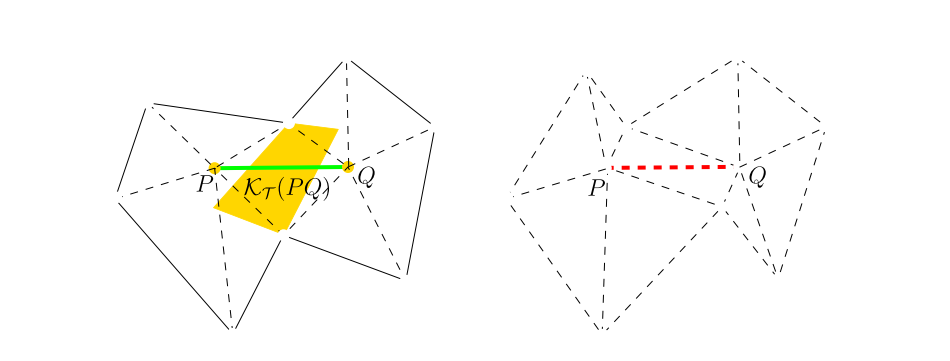
\includegraphics[width=\textwidth]{kernel_area}
    \caption{kernel area}
    %\label{fig:three sin x}
  \end{subfigure}
  %\caption{constratint}
  %\label{fig:three graphs}
\end{figure}
\end{frame}

%------------------------------------------------
%\section{Second Section}
%------------------------------------------------

\begin{frame}
\frametitle{Simplicication}
\begin{block}{Other two kind of edge collapse}
First perform a mutual tessellation between $\mathcal{Z}$ and $\tau$.
Then do two kinds of edge collapse, with the same as constratint as above, the third constraint can also say, each edge of the target point linked should not intersect with $\partial \Gamma$:
\begin{itemize}
  \item edge collapse of edges in $\mathcal{Z}$ (high priority)
  \item edge collapse between $\mathcal{Z}$ and $\partial \Gamma$
\end{itemize}
\end{block}
\begin{figure}[h]
  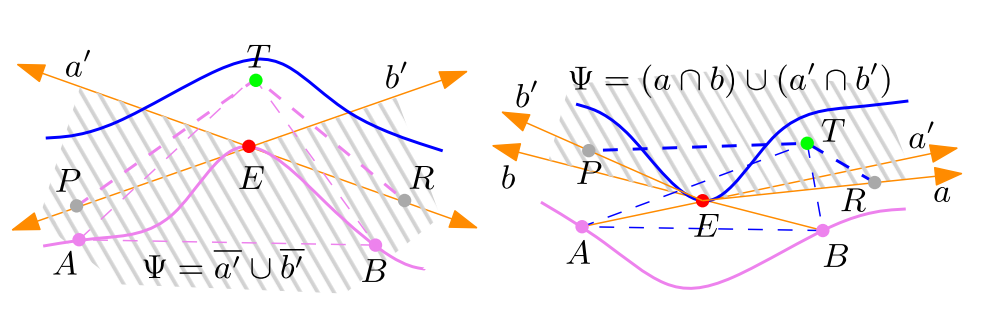
\includegraphics[width=8cm]{ec_z}
\end{figure}
\end{frame}

%------------------------------------------------
%----------------------------------------------------------------------------------------

\end{document} 
